\chapter{Automatisation de la maison}

\section{L’intelligence des objets}
	\subsection{Définition d’un objet connecté}
Aujourd'hui les objets connectés font partis de notre quotidien, et peuvent réaliser énormément 
d'actions différentes. Globalement on peut dire qu'un objet connecté, ou l'internet des objets, représente 
l'extension d'Internet à l'ensemble des objets de notre monde physique. Cela permet de donner de 
l'intelligence à des objets, afin qu'ils puissent nous communiquer différentes informations 
(\textbf{Capteurs}), ou bien exécuter différentes choses (\textbf{Actionneurs}). Ces événements peuvent être 
réalisés manuellement ou automatiquement selon le besoin.

Malgré tout, ces objets ne sont sémantiquement pas connectés entre eux pour plein de raisons différentes. 
SmartDevCom permet de réaliser un ensemble d'objet tous connectés entre eux. Un objet connecté est constitué 
d'un ou plusieurs capteur(s) ou actionneur(s).
% 		Définition générale + notre version par rapport au projet
	\subsection{Les capteurs}
	
Les capteurs sont tous les objets qui permettent d'obtenir une information sur l'environnement. Ces capteurs 
permettent par exemple de connaître la température de la pièce, de savoir si la lumière est allumée, ou si la 
porte d'entrée est ouverte.

Ces capteurs permettent une interaction simpliste avec l'environnement puisqu'ils permettent seulement 
d'obtenir une information physique. Ainsi, l'utilisation d'un capteur est très simple, puisqu'il suffit de 
lui demander d'envoyer la valeur qu'il contient.
% 		les types de capteurs
% 		leurs caractéristiques au sein d’un objet connecté
	\subsection{Les actionneurs}
	
Les actionneurs sont tous les objets qui permettent de réaliser une action. Ces actionneurs permettent par 
exemple d'ouvrir les volets, d'allumer la climatisation, ou bien d'allumer la lumière.

Ils permettent une interaction plus prononcée avec l'environnement, comparativement aux capteurs, étant donné 
qu'ils ont besoin de paramètres pour réaliser l'action voulue. Par exemple si l'on souhaite allumer une 
lumière intelligente, il faudra préciser l'intensité lumineuse, ainsi que la couleur de celle-ci.
% 		les types de capteurs
% 		leurs caractéristiques au sein d’un objet connecté

\section{La communication des objets}
	\subsection{Présentation des technologies de communication}
Actuellement, il existe de nombreux protocoles réseaux qui permettent la communication entre les différents 
objets. Ces protocoles établissent des normes, afin de pouvoir dialoguer entre différents acteurs.

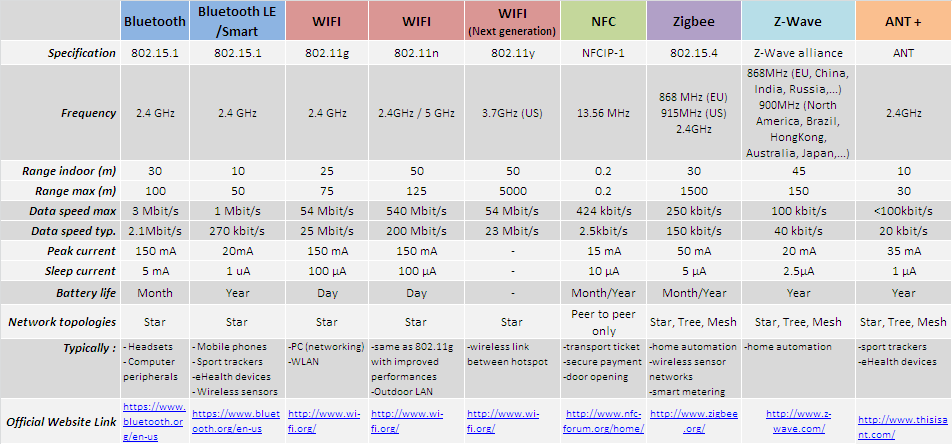
\includegraphics{img/tableau-total.png} 

Tous ces protocoles ont leur avantages et leur inconvénients. Malgré tous ces protocoles, on peut voir qu'il 
existe principalement deux familles :

\paragraph{Les protocoles très énergivores}qui permettent de faire transiter des données avec un débit très 
élevé. Cette cadence est permise grâce à une fréquence trés élevé. Cette fréquence a par conséquent 
l'inconvénient de très peu passer les obstacles, et donc d'émettre sur une courte distance.

\paragraph{Les protocoles peu énergivores}qui possèdent des caractéristiques opposées. En effet ils 
permettent de faire transiter des données avec un faible débit, sur une grande distance grâce à une fréquence 
bien moindre.

C'est donc la deuxième famille qui est la plus utilisée pour l'internet des objets, puisqu'ils n'ont pas 
besoin d'envoyer beaucoup de données, ont besoin d'envoyer le plus loin possible, et surtout d'avoir le plus 
d'autonomie possible. Les protocoles les plus réprésentatifs de cette famille, sont le Bluetooth Low Energy 
(ou BLE), le Zigbee, et Z-Wave. Ces deux derniers sont relativement onéreux et compliqués à mettre en place, 
c'est pourquoi le BLE est le protocole le plus démocratisé de cette famille.

% 		wifi, bluetooth, BLE, zig-bee, …
% 		quelques caractéristiques (débit, portée, consommation)
	\subsection{Les différentes topologies de réseaux}
En plus des différents protocoles, il existe aussi des topologies différentes pour créer un réseau d'objets.

	    \subsubsection{Etoile}
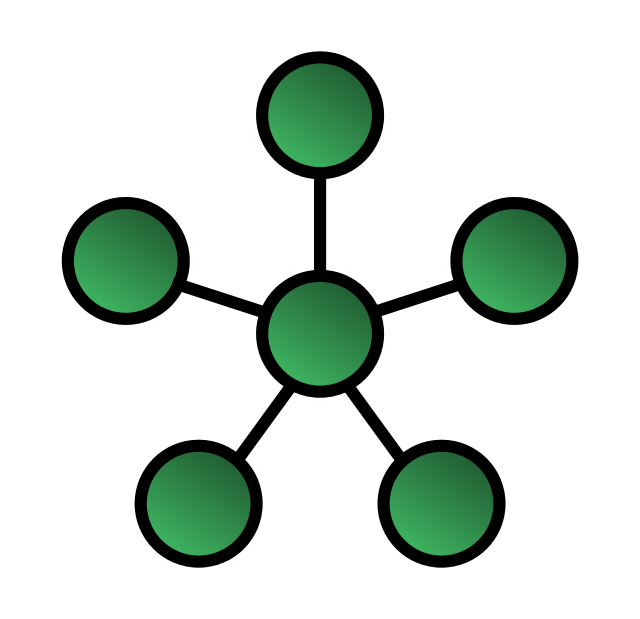
\includegraphics{img/StarNetwork.svg.png}

	    \subsubsection{P2P}
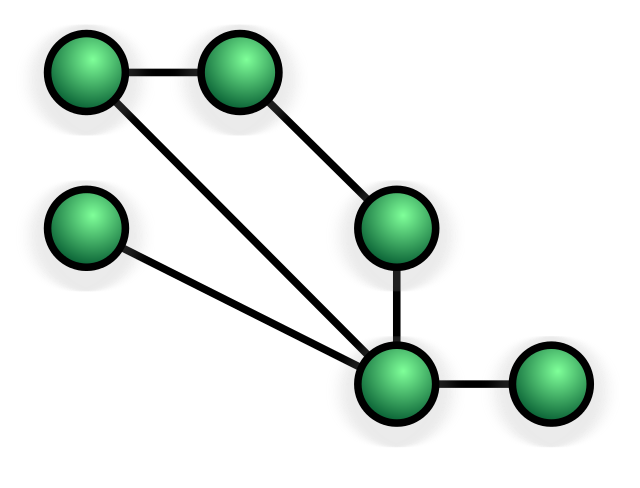
\includegraphics{img/NetworkTopology-Mesh.svg.png}

	    \subsubsection{Arbre}
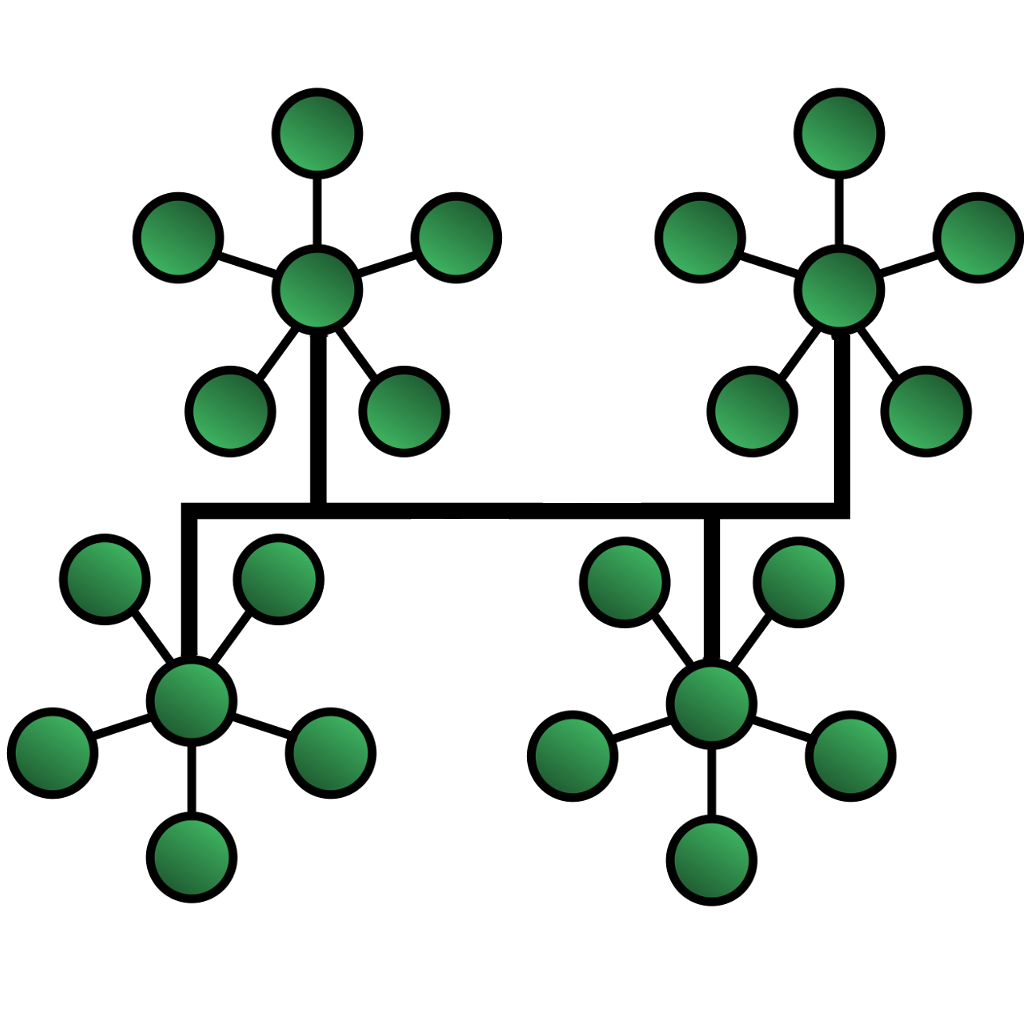
\includegraphics{img/TreeTopology.png}


% 		p2p, étoile, mesh, ...
% 		lien avec les technos
	\subsection{Application du réseau à la domotique}
% 		les technologies les plus adaptées à la domotique
% 		exemples d’architecture réseau dans une maison (avec ou sans mélange de technos)

\section{La centralisation de l’intelligence : Jarvis}
	\subsection{Vision macroscopique d’un système domotique}
% 		les conséquences de la connexion des objets
	\subsection{Les scénarios}
% 		explication sur l’intérêt de la connexion des objets
% 		exemples d’utilisations
	\subsection{Analyse et anticipation de requêtes}
% 		analyse plus poussée des données : statistiques, interprétations des mesures
% 		intégration d’intelligence artificielle
% 		exécution de tâches de façon autonomes
% 		les limites
